\section{Digitaltechnik}
Die \textbf{CMOS} Logik gegenüber Bipolar-Transistoren haben \underline{keinen statischen Stromverbrauch}, \underline{hohe Störsicherheit}, brauchen aber \underline{mehr Transistoren}. Alle CMOS-Schaltungen haben IMMER einen Pull-UP (PUP, PMOS, Verbindet bei 0 und öffnet bei 1) und Pull-Down (PDN, NMOS, Verbindet bei 1 und öffnet bei 0) teil!

\noindent\textbf{Beispiel} eines komplexen CMOS Schaltung. Alle möglichen Zustände müssen definiert sein und keiner darf Floating sein. Das bedeutet, dass jede PMOS und NMOS Logikteil immer Dual zu einander sein müssen und immer genau einen Pfad hat $\xRightarrow{}$ Serie zu Parallel, Parallel zu Serie.
\begin{center}
	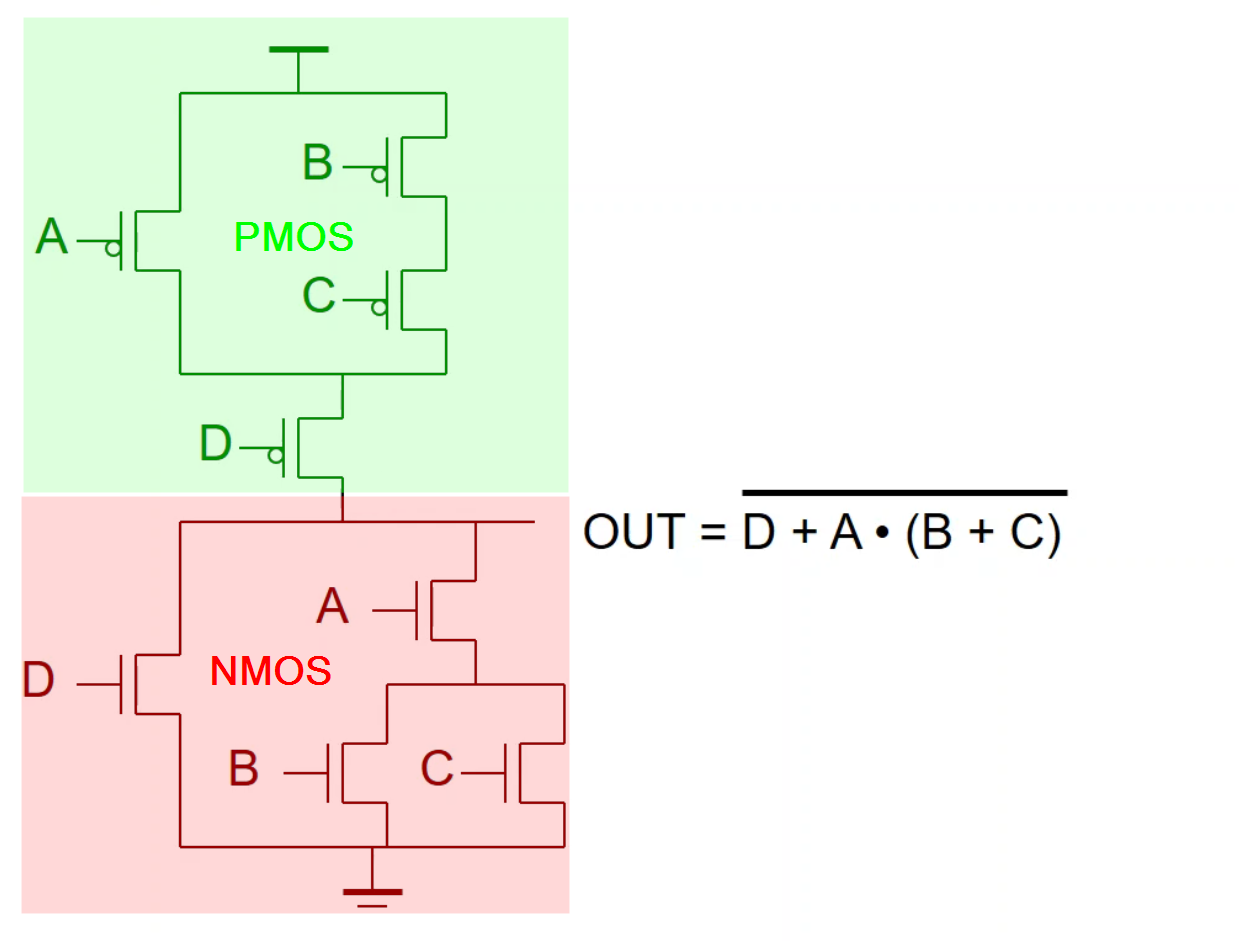
\includegraphics[width=\columnwidth]{Images/cmos}
\end{center}

\subsection{Verzögerungszeit CMOS}
Bei MOSFET als \textbf{Widerstand} ergibt sich die Verzögerungszeit mit Technologieparameter $R_{on}, C_L, V_{swing}, I_{AC}$ als
\[
t = \ln(0.5)\cdot R_{on}C_L
\]
Mit Stromquelle
\[
t = \frac{C_L \frac{V_{swing}}{2}}{I_{AV}}
\]
Aus diesen Gründen ist bei ähnlicher Technologe-Dimension Bipolar schneller als MOS.

\subsection{Spannungspegel}
\begin{center}
	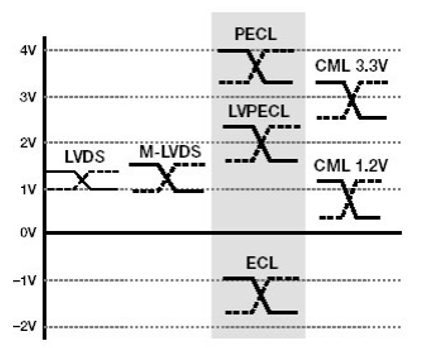
\includegraphics[width=0.8\columnwidth]{Images/spannungspegel}
\end{center}


\subsection{Signalübertragung}
\begin{center}
	\includegraphics[width=0.8\columnwidth]{Images/signalübertragung}
\end{center}

